\documentclass[a4paper,12pt]{ctexart}
\usepackage{amsmath}
\usepackage{amsfonts}
\usepackage{float}
\usepackage{enumerate}
\usepackage{svg}
\usepackage{graphicx}
\usepackage{booktabs}
\usepackage[hidelinks]{hyperref}
\usepackage[scale=0.8]{geometry}
\usepackage{ulem}
\setcounter{secnumdepth}{0}
\setlength{\abovecaptionskip}{3pt}
\setlength{\belowcaptionskip}{0pt}
\title{以澜起科技(688008.SH)换兆易创新(603986.SH)}
\author{董晨阳}
\date{\today}
\begin{document}
\maketitle
\thispagestyle{empty}
\begin{abstract}
    \textbf{澜起科技和兆易创新都是Fabless的存储厂商,将芯片制造外包给Foundry厂商,但二者侧重点有所不同}。澜起科技主要做DRAM的内存接口芯片,互联类芯片还做DDR5配套芯片、PCIe Retimer芯片和CXL控制芯片,此外还有津逮服务器平台包装Intel CPU和安全性模块。兆易创新则是做NOR Flash,此外还有MCU和传感器业务。

    看好澜起科技的因素有:1)\textbf{澜起科技在半导体周期中有更强的beta}。半导体周期如若反转,DRAM的弹性最大。若AI启动了半导体需求周期,高性能服务器上内存缓冲芯片必不可少,这部分增量将几乎全部作用到澜起科技等少数几家企业。2)\textbf{竞争格局优,且具备竞争优势}。内存缓冲芯片目前仅有三家企业,新企业难以进入。澜起有一定的技术优势,引领了标准制定,且Intel作为股东对其技术的认证有利于澜起打下市场空间。3)\textbf{DDR5渗透可能进一步提升竞争力}。澜起DDR5技术更完备,DDR5渗透可能带动其ASP提升。

    看淡兆易创新的因素有:1)\textbf{半导体周期中NOR Flash弹性不大},本轮半导体周期的需求周期可能不是由IoT及汽车电子引领。2)利基市场具备竞争优势,但收购上海思立微商誉存在\textbf{商誉减值风险}。3)\textbf{制裁风险}。董事长兼任合肥长鑫董事长,长鑫被美国制裁,为兆易创新代工的DRAM难以高端化带来利润且产能有限,且兆易创新也有被进一步制裁的风险。

    估值方面,假定23年底周期启动,24年估值回升至上一周期30-40\%分位,预测澜起科技2024 EPS 1.23元,给予PE65-71x,目标价80-87元,上行空间27\%-39\%;预测兆易创新2024 EPS 2.68元,给予PE34-50倍,目标价91-142元,对应上行空间-17\%-28\%。

    \textbf{风险提示}:议价能力减弱,研发不及预期,周期未启动,汽车电子及IoT设备超预期繁荣
\end{abstract}
\clearpage
\tableofcontents
\listoffigures
\clearpage
\setcounter{page}{1}
\section{公司业务对比:不同赛道的存储厂商}

\subsection{澜起科技:内存互联为主,计算类产品为辅}
\textbf{澜起科技成立于2004年,与Intel有很深的联系}。澜起科技业务主要是内存接口芯片,2006年澜起的DDR2接口芯片成功获得Intel青睐和入股,自从DDR4世代及之后澜起在内存接口芯片市场上占据了领先优势,\uline{跟随并影响}DDR标准迭代,并在随后沿着计算机内部硬件互联的路线研发出PCIe Retimer芯片和CXL控制芯片等。此外,澜起还和Intel合作开发了津逮CPU与服务器,做到一定程度的可控。
\begin{figure}[H]
    {\centering
        \caption{澜起科技发展历程}
        \includegraphics[width=\linewidth]{img/history-lq.png}
        \par}
    \footnotesize{资料来源:公司公告}
\end{figure}

\textbf{内存接口芯片处于服务器产业链上游,连接CPU与DRAM}。DRAM是真正意义上的“内存”,计算机运行时的数据在DRAM内供CPU使用、调度,断电就会丢失数据。DRAM的标准是DDR,最新为DDR5。DRAM速度(MHz级)比CPU(GHz级)慢,内存接口芯片来缓冲一部分DRAM数据给CPU调度。因此内存接口芯片也称为内存缓冲芯片,在DDR4及之前仅用于高端的服务器,DDR5(及之后)也可供应PC、笔电。DDR5需要许多配套芯片,如电源管理PMIC、温度传感器TS等,澜起科技也提供这些配套芯片,但不提供GDDR或是HBM相关产品。
\begin{figure}[H]
    \begin{minipage}{0.48\linewidth}
        \centering
        \caption{内存接口芯片的位置}
        \includegraphics[width=0.8\linewidth]{img/illustration.png}
    \end{minipage}
    % TODO
    \begin{minipage}{0.48\linewidth}
        \centering
        \caption{产业链分工}
        \includegraphics[width=0.8\linewidth]{img/chain.png}
    \end{minipage}\par
    \footnotesize{资料来源:Rambus}
\end{figure}
\textbf{内存接口芯片原理是缓存,相当于CPU三级缓存(SRAM)的缓存}。内存接口芯片主要包括寄存缓冲器(Register Clock Driver,RCD)和数据缓冲器(Data Buffer,DB),分别用来缓冲来自内存控制器的控制信号和来自内存控制器或DRAM的数据信号。仅采用了RCD芯片的内存模组(DIMM)通常称为 RDIMM,而采用了 RCD 和 DB 套片的内存模组称为LRDIMM,二者主要用于服务器。
\begin{figure}[H]
    \caption{RDIMM与LRDIMM图示}
    \begin{minipage}{0.48\linewidth}
        \centering
        \includegraphics[width=\linewidth]{img/rdimm.png}
    \end{minipage}
    \begin{minipage}{0.48\linewidth}
        \centering
        \includegraphics[width=\linewidth]{img/lrdimm.png}
    \end{minipage}\par
    \footnotesize{资料来源:Rambus}
\end{figure}

\textbf{内存接口芯片的下游主要是DRAM厂商,再往下是高端服务器}。就分工而言,内存接口芯片属于逻辑芯片,功能更多的是数据的处理和CPU的对接,存储厂商并不善于此,通常从外部采购,与DRAM等组装成内存模组再卖给下游服务器厂商。这些内存模组RDIMM/LRDIMM主要用在高端服务器上以充分利用服务器上的大内存、获取更高的性能。

\textbf{其他互联类业务方面,澜起还研发了PCIe Retimer芯片和CXL控制芯片}。PCIe与CXL都是传输协议,其中CXL较新,应用并不多。PCIe Retimer能减少信号随距离产生的衰减,从而提升传输的质量,广泛用于计算机内部的连接,如CPU与GPU、硬盘等的连接。
\begin{figure}[H]
    {\centering
        \caption{PCIe Retimer的应用场景}
        \includegraphics[width=0.8\linewidth]{img/PCIe 4.0 Retimer Application_CH.jpg}\par}
    \footnotesize{资料来源:公司官网}
\end{figure}

\textbf{计算类业务澜起的津逮服务器使用了Intel的Xeon CPU,加入了安全性模块}。安全性模块可以通过芯片级实时安全监控功能,动态排查CPU的异常行为,保障服务器的安全,一定程度上做到了“自主可控”。津逮服务器也积极配合国产的其他硬件和软件,2022年贡献了约35\%的收入,但毛利率较低,仅为10\%。

\subsection{兆易创新:NOR Flash切入低端存储,辅以MCU、传感器}

% 1页
\textbf{兆易创新的存储以NOR Flash见长,NAND与DRAM面向利基市场}。闪存Flash断电数据不易失。其中NAND Flash更便宜、容量和市场空间更大,主要用作存数据的“硬盘”,兆易创新做的是其中利基市场上2D的SLC NAND。NOR Flash约占整个存储市场规模的2\%,也是一个利基市场,曾广泛用于功能机。尽管NOR Flash容量小,但其上能执行代码,现在主要用在IoT设备和汽车电子领域,兆易创新的市场份额约20\%,存储营收超70\%为NOR。DRAM由长鑫存储代工,主要面向利基市场,如机顶盒和车载影音系统。
\begin{figure}[H]
    {\centering
        \caption{半导体市场细分(USD),黄色为澜起所位置,红色及DDR4为兆易创新所在位置}
        \includegraphics[width=\linewidth,trim=0 0 0 80]{img/semi.png}\par}
    \footnotesize{资料来源:WSTS}
\end{figure}

\textbf{除了NOR Flash外,兆易创新收入主要由MCU和传感器贡献}。微控制器MCU在汽车电子、工业设计、消费电子等方面都必不可少。近年来汽车新能源化水平提升,一辆智能汽车需要的MCU数量(约300个)远高于传统燃油车(约70个),全球MCU车用占比从2018年的35\%增长到了2021年的约40\%。MCU成为兆易创新增长的动力源之一。
\begin{figure}[H]
    \begin{minipage}{0.48\linewidth}
        \caption{NOR在IoT和汽车带领下复苏}
        \centering
        \includegraphics[width=\linewidth]{img/norflash.png}
    \end{minipage}
    \begin{minipage}{0.48\linewidth}
        \caption{车用MCU占比提升}
        \centering
        \includegraphics[width=\linewidth]{img/mcu.png}
    \end{minipage}\par
    \footnotesize{资料来源:Wind,ASPENCORE,JW Insight}
\end{figure}

\section{行业beta:半导体周期中DRAM弹性更大,利好澜起}
% 2页
\textbf{全球半导体行业每隔 4-5 年经历一轮周期,国内半导体的周期性与全球半导体周期基本同步}。从谷到峰的上行周期通常 1-3 年时间,从峰到谷的下行周期通常 1-2 年时间。\uline{费城半导体指数(SOX)修复往往由于存在预期博弈领先于基本面(半导体销售额)的改善}。半导体作为全球分工的产业,我国半导体在国产替代的旋律之外也随周期波动。
\begin{figure}[H]
    {\centering
        \caption{复盘半导体周期,三家公司股价(相对值)启动后的表现,DXI为DRAM价格指数}
        \includegraphics[width=0.8\linewidth]{img/sox.png}\par}
    \footnotesize{资料来源:Wind}
\end{figure}

\textbf{复盘周期有各自不同的一或多Trigger、类似的DRAM/设备/硅片/Foundry产能利用率等景气循环}。每轮周期的启动看似多种原因,例如4G与智能手机兴起、云计算流行、疫情提升线上生活比例。但每轮周期都有类似的现象,其中DRAM由于标准化且总量大(逻辑电路能拆解出种类繁多的CPU、ASIC等)、几乎所有电子产品都必须用到一定数量(NOR只有部分用到,NAND硬盘可以节省)、玩家少、短期产能有限,周期中弹性是最大的。
\begin{figure}[H]
    \caption{DRAM弹性大且和SOX更相关,NAND相关性弱一些}
    \begin{minipage}{0.48\linewidth}
        \centering
        \includegraphics[width=\linewidth]{img/monthly.png}
    \end{minipage}
    \begin{minipage}{0.48\linewidth}
        \centering
        \includegraphics[width=\linewidth]{img/quarterly.png}
    \end{minipage}\par
    \footnotesize{资料来源:Wind,macromicro}
\end{figure}
\subsection{周期的成因:供给、库存与需求共振}
\textbf{供需周期错配带来半导体周期波动}。\uline{半导体的需求周期是不可预测的}。许多Trigger都有可能成为需求周期爆发的起点,成功者有智能手机、云计算等,但也有暂时没有引爆需求的案例,例如元宇宙、VR、汽车电子。此外,\uline{半导体的供给周期是不灵活的}。前期需要极高的Capex,Capex与公司业绩和景气度相关,并且建一条产线的时间(2-4年)可能跨越一个周期;产能建成后利用率有上限,且技术在不断革新,例如摩尔定律、DDR代数等。对于高度集中且标准化的DRAM,IDM玩家单独的决策对供给的影响也非常大,加剧了供给的不灵活性;但IDM为主也意味着产业链更短,DRAM价格与股价/SOX更贴近。
\begin{figure}[H]
    \begin{minipage}{0.48\linewidth}
        \caption{DRAM集中于前三家IDM}
        \centering
        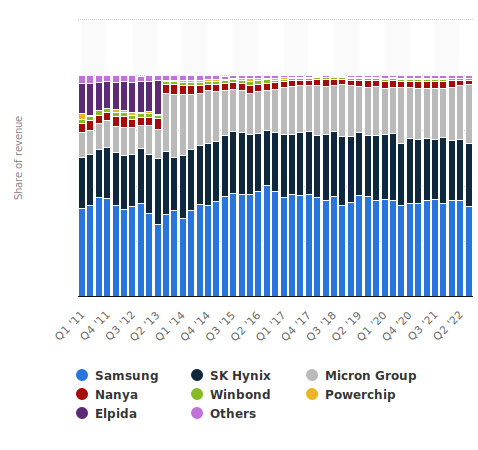
\includegraphics[width=\linewidth]{img/dram.png}
    \end{minipage}
    \begin{minipage}{0.48\linewidth}
        \caption{NOR Flash与NAND相对分散}
        \centering
        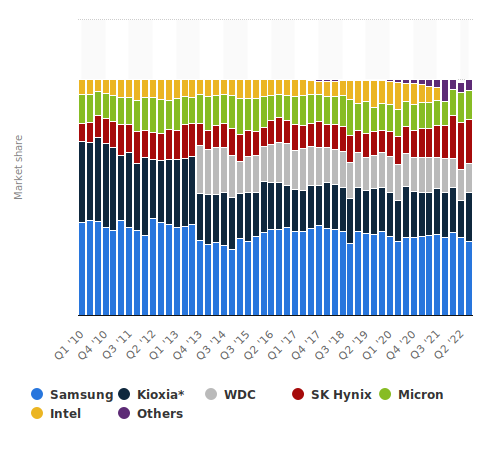
\includegraphics[width=\linewidth]{img/nand.png}
    \end{minipage}\par
    \footnotesize{资料来源:Statista}
\end{figure}

\textbf{库存平抑供需波动的作用不明显,有时反而加剧了周期波动}。半导体产业内Fabless+Foundry的产业分工使各Fabless都需要预测需求、备库存以防抢不到产能,层层库存与预测的偏差可能导致库存高企超出需求,导致下跌更惨烈(尔必达)。

\subsection{本轮周期推演:服务器、DRAM景气程度高,澜起beta更强}

\textbf{当前半导体处于下行周期,但存在即将反转迹象}。2022年全球高通胀、国内疫情、疫情需求透支使整体需求疲软,库存处于相对高位,迫使存储厂商减产DDR4、台积电产能利用率仅7成、消费电子哀鸿遍野、ASML订单新低等,行业主动去库存。但当前AI产业链上的Nvidia数据中心显卡与Hynix HBM显存等已经进入了被动去库存乃至主动补库存阶段,DRAM价格有上升势头。很难预测准具体的反转时间,台积电等企业预期23下半年反转。

\textbf{AI可能成为本轮周期的Trigger,景气可能从高性能计算服务器开始传导}。服务器需要的是DRAM而非NOR Flash,高性能服务器上DRAM需求更大且内存缓冲芯片必不可少,否则性能将严重下降,这部分增量将几乎全部作用到澜起科技等少数几家企业,因此行业beta方面更看好澜起科技。

\section{个股alpha:澜起内存接口芯片增长空间更优}
% 3页
% \subsection{共同的主线:国产替代}
\textbf{周期性之外,国产替代是我国半导体产业的另一条趋势,澜起与兆易各自均有布局}。澜起的津逮服务器近年营收快速增长,利用了Intel高性能的同时,保证信息的自主可控。这种思路能最大程度地复用x86生态,并且性能保持强劲,但是核心技术并非自主化,更适合在国产替代早期替代一些性能敏感的场景,1Q23可以看到其收入大幅下降98\%,\uline{对其不应有过高期待}。兆易核心技术为国产,NOR Flash与MCU技术相对领先,虽然DRAM受限于制程等因素较国际先进水平仍有差距,但利基市场战略使兆易创新替代能力更强。
\begin{figure}[H]
    \begin{minipage}{0.48\linewidth}
        \caption{澜起科技分产品主营收入}
        \centering
        \includegraphics[width=\linewidth]{img/lqkj-rev.png}
    \end{minipage}
    \begin{minipage}{0.48\linewidth}
        \caption{兆易创新分产品主营收入}
        \centering
        \includegraphics[width=\linewidth]{img/zycx-rev.png}
    \end{minipage}\par
    \footnotesize{资料来源:Wind}
\end{figure}

\subsection{澜起科技:技术领先具有竞争优势,DDR5渗透进一步提升竞争力}

\textbf{内存接口芯片市场高度集中,进入壁垒高、缺乏替代品,澜起在现存竞争者中具有一定的竞争优势}。内存接口芯片需要功耗低且工作快,自DDR4世代开始,行业主要参与者仅剩澜起、瑞萨(IDT)、Rambus三家。供给侧,澜起参与了DDR标准制定,2013年发明的“1+9”框架(1个RCD和9和DB)成为了2014年JEDEC的DDR4 LRDIMM标准。需求侧,除了与现有DRAM厂商良好合作外,由于内存接口芯片认证过程严格,需要CPU公司、内存公司的多重认证,其中尤以CPU厂商认证最为关键;而Intel作为股东对其技术的认证有利于澜起打下市场空间,例如其“1+9”架构早在2013年便被Intel认证了。
\begin{figure}[H]
    \begin{minipage}{0.48\linewidth}
        \caption{内存接口芯片各世代主要厂商}
        \centering
        \includegraphics[width=\linewidth]{img/ddr.png}
    \end{minipage}
    \begin{minipage}{0.48\linewidth}
        \caption{澜起自DDR4起市占率快速提升}
        \centering
        \includegraphics[width=0.9\linewidth]{img/mktshare.png}
    \end{minipage}
    \par\footnotesize{资料来源:华经产业研究院,Wikipedia}
\end{figure}
\textbf{就买卖方议价能力而言,澜起表现相对强势}。尽管DRAM也是寡头垄断的格局,但从应收应付的角度看,澜起股份应收和应付占比都不高,且互联类芯片业务毛利率相对稳定在60\%以上(2022年起DDR5配套芯片出货拉低毛利率)。这可能是由于内存接口芯片垄断程度更高,而几大内存厂之间竞争更为激烈。
\begin{figure}[H]
    \begin{minipage}{0.48\linewidth}
        \caption{澜起科技毛利率}
        \centering
        \includegraphics[width=\linewidth]{img/lqmargin.png}
    \end{minipage}
    \begin{minipage}{0.48\linewidth}
        \caption{澜起科技应收应付占总资产比例}
        \centering
        \includegraphics[width=\linewidth]{img/ysyf.png}
    \end{minipage}
    \par\footnotesize{资料来源:Wind}
\end{figure}

\textbf{市场空间方面,DDR5的渗透可能让澜起科技优势进一步提升}。当前需要额外配套芯片的DDR5逐步取代DDR4,Yole预计2024年DDR5出货将超过DDR4,其可能的影响包括:首先,澜起竞争优势可能更加稳固,因为IDT 实力强劲,但2018年被瑞萨收购后重心放在在模拟混合信号领域(见\href{https://www.renesas.cn/cn/zh/about/press-room/integrated-device-technology-start-operations-renesas-electronics-america-january-2020-following}{链接}),内存接口芯片战略地位有所下降,未来市占率可能继续降低;Rambus 技术也很强,但DB及DDR5的配套芯片(见\href{https://www.rambus.com/memory-and-interfaces/server-dimm-chipsets/ddr5-dimm-chipset/}{链接})相对还未完善,在DDR5时代很难赶超澜起科技和IDT。其次,DDR5标准下,PC及笔记本电脑也可以使用内存接口芯片,可能会带来一定的增量。最后,如同DDR4内部不同Gen迭代使得澜起ASP逐步提升,DDR5子代迭代也可能进一步提升澜起的ASP(因出货DDR5配套芯片,ASP拉低)。
\begin{figure}[H]
    \begin{minipage}{0.48\linewidth}
        \caption{DDR5出货量占比逐步提升}
        \centering
        \includegraphics[width=\linewidth]{img/ddr5.jpeg}
    \end{minipage}
    \begin{minipage}{0.48\linewidth}
        \caption{澜起科技互联类芯片ASP}
        \centering
        \includegraphics[width=\linewidth]{img/asp.png}
    \end{minipage}
    \par\footnotesize{资料来源:Wind,Yole Developments}
\end{figure}

\textbf{AI芯片为公司打开了想象空间}。澜起深耕内存和CPU的连接,有助于AI芯片处理内存墙的问题,第一代AI芯片样片已于2022年底完成流片,\textbf{但走到量产仍有不确定性}。
\subsection{兆易创新:下游需求可能放缓,存在制裁风险}
\textbf{兆易创新在存储的利基市场以及MCU上有一定的竞争优势}。NOR Flash主流制程为55nm,且传统厂商如美光、Cypress等退出了低端产品,两家台湾厂商以高端消费电子产品为主,兆易创新在汽车电子和低端消费电子领域打下了市场份额,再向中高端产品延伸。DRAM从代销长鑫产品转为长鑫代工自有产品\footnote{兆易创新创始人兼董事长朱一明兼任长鑫董事长,兆易创新持有长鑫母公司1.26\%股份。22年10月起美国禁止18nm以下DRAM制造设备出口到中国、长鑫被列入实体清单,23年1月长鑫裁员;兆易暂时没有被制裁,但\textbf{存在被制裁的风险}},产品制程17和19nm,但受制于长鑫被制裁,该部分产能有限。MCU方面可以对标意法半导体“MCU百货超市”,型号丰富且大量产品通过了车规级认证,工业及汽车MCU占比已达50\%,贡献了大量毛利。
\begin{figure}[H]
    \begin{minipage}{0.48\linewidth}
        \caption{兆易创新NOR市场份额}
        \centering
        \includegraphics[width=\linewidth]{img/nor.png}
    \end{minipage}
    \begin{minipage}{0.48\linewidth}
        \caption{MCU毛利率相对较高}
        \centering
        \includegraphics[width=\linewidth]{img/margin.png}
    \end{minipage}
    \par\footnotesize{资料来源:Cinno Research}
\end{figure}

\textbf{市场空间方面,兆易创新过去的增长点难以持续高增长}。2017-2019年传统大厂退出、TWS耳机等IoT设备兴起,NOR Flash结束了功能机时代起的萎缩,兆易创新抓住机会从低端消费电子起家。2020年至今新能源汽车蓬勃发展,全线带动了MCU、NOR Flash和传感器的需求。目前尽管新能源车结构性替代传统燃油车的趋势不变,但增速受基数效应及宏观消费的影响趋缓,且汽车整体产销量处于下降趋势。
\begin{figure}[H]
    \caption{燃油车销量疲软,新能源车销量增速放缓}
    \begin{minipage}{0.48\linewidth}
        \centering
        \includegraphics[width=\linewidth]{img/car11.png}
    \end{minipage}
    \begin{minipage}{0.48\linewidth}
        \centering
        \includegraphics[width=\linewidth]{img/car2.png}
    \end{minipage}
    \par\footnotesize{资料来源:中汽协}
\end{figure}

\section{财务对比与估值分析:澜起上升空间更大}
收入和利润方面,二者毛利率、费用率和净利率接近,兆易的收入与毛利约为澜起的两倍。澜起收入以国外为主,在引入津逮(毛利率10\%)后毛利率从60\%下滑至45\%。兆易收入以国内为主,自2020年起高毛利MCU快速上量,20、21年MCU收入同增63\%、106\%,21年MCU收入占比29\%而毛利占比41\%。二者费用结构相似,均为重研发、轻营销,但兆易财务费用更低,因此营业利润率分别为29\%和33\%。
\begin{figure}[H]
    \centering
    \begin{minipage}{0.48\linewidth}
        \caption{澜起科技收入毛利}
        \centering
        \includegraphics[width=\linewidth]{img/lq1.png}
    \end{minipage}
    \begin{minipage}{0.48\linewidth}
        \caption{兆易创新收入毛利}
        \centering
        \includegraphics[width=\linewidth]{img/zy1.png}
    \end{minipage}
    \begin{minipage}{0.48\linewidth}
        \caption{澜起科技费用率与利润率}
        \centering
        \includegraphics[width=\linewidth]{img/lq2.png}
    \end{minipage}
    \begin{minipage}{0.48\linewidth}
        \caption{兆易创新费用率与利润率}
        \centering
        \includegraphics[width=\linewidth]{img/zy2.png}
    \end{minipage}
\end{figure}
自由现金流和资产方面,两家公司自由现金流均有波动,兆易创新的波动更大。兆易创新2019年溢价19倍(17亿)收购了做传感器的思立微,存在较高比例的商誉,有减值风险。
\begin{figure}[H]
    \begin{minipage}{0.48\linewidth}
        \caption{两家公司FCFF(百万元)}
        \centering
        \includegraphics[width=\linewidth]{img/fcf.png}
    \end{minipage}
    \begin{minipage}{0.48\linewidth}
        \caption{兆易创新商誉}
        \centering
        \includegraphics[width=\linewidth]{img/goodwill.png}
    \end{minipage}
\end{figure}
估值方面,考虑半导体周期反转可能会给股价带来戴维斯双击,当前澜起科技和兆易创新的PE(TTM)仍在近一个半导体周期(2020-2023)15\%分位点。若假定23H2内周期启动,两家公司23年营收均可能下滑、24年恢复,毛利率均承压。而由于澜起弹性更高,周期启动后恢复更快,预测全年收入下滑不大。2024 PE修复至30/40\%分位点,则2024年估值如下表所示。预计兆易创新上升空间-19\%-26\%,澜起科技上升空间27\%-39\%。
\begin{figure}[H]
    \begin{minipage}{0.48\linewidth}
        \caption{澜起科技PE(TTM)}
        \centering
        \includegraphics[width=\linewidth]{img/pe-lq.png}
    \end{minipage}
    \begin{minipage}{0.48\linewidth}
        \caption{兆易创新PE(TTM)}
        \centering
        \includegraphics[width=\linewidth]{img/pe-zy.png}
    \end{minipage}
\end{figure}
\begin{table}[H]
    \caption{估值分析}
    \centering
    \begin{tabular}{|l|rr|r|rr|r|rr|}
        \hline
             & \multicolumn{2}{c|}{24年PE} & \multicolumn{1}{c|}{EPS} & \multicolumn{2}{c|}{对应} & \multicolumn{1}{c|}{当前} & \multicolumn{2}{c|}{空间}                                                    \\ \hline
        兆易创新 & \multicolumn{1}{r|}{34}    & 53                       & 2.679                   & \multicolumn{1}{r|}{91} & 142                     & 112.48 & \multicolumn{1}{r|}{-19.03\%} & 26.22\% \\ \hline
        澜起科技 & \multicolumn{1}{r|}{65}    & 71                       & 1.230                   & \multicolumn{1}{r|}{80} & 87                      & 63.04  & \multicolumn{1}{r|}{26.83\%}  & 38.54\% \\ \hline
    \end{tabular}
\end{table}
\begin{figure}[H]
    \begin{minipage}{0.48\linewidth}
        \caption{澜起科技财务预测(百万元)}
        \centering
        \includegraphics[width=\linewidth]{img/valuation-lq.png}
    \end{minipage}
    \begin{minipage}{0.48\linewidth}
        \caption{兆易创新财务预测(百万元)}
        \centering
        \includegraphics[width=\linewidth]{img/valuation-zy.png}
    \end{minipage}
\end{figure}
\subsection{潜在风险}
\begin{enumerate}
    \item 澜起客户集中度进一步提升,下游议价权上升,应收增加、价格下降。
    \item 新技术如DDR6等未能跟上或研发不及预期。
    \item 半导体周期启动更晚,或预期一致导致行业内部压库存到年底释放,盈利持续下降。
    \item 汽车电子及IoT设备超预期繁荣。
\end{enumerate}

\end{document}
